\chapter{Technical Risk Analysis}
\label{ch:Technical_Risk_Assessment}
This chapter performs a proper technical risk analysis to assess the \textit{Swing eVTOL} extensively.
Firstly, in \Cref{sec:tech_risks}, the risk likelihood and impact metrics are defined, as well as the risks themselves.
Subsequently, the mitigation strategies and contingency plans are established in \Cref{sec:mitandcont} to improve the risk maps
(\Cref{fig:Risk_map}).

\section{Technical Risks}
\label{sec:tech_risks}
To identify and quantify risks correctly,
in \Cref{tab:likelihood_metrics,tab:impact_metrics}, the following risk metrics for likelihood and impact are used.
Through the use of these metrics, a well-defined risk analysis can be performed,
multiplying each risk’s likelihood and impact, then dividing it by five to retrieve the risk factor.
\Cref{tab:tech_risk_analysis} establishes all the technical risk, each consisting of a risk ID,
the main risk period, and a description of both risk and its impact.
The risk ID contains the category, period, and chronological numbering in its ID,
which will be mainly used for the identification in the risk maps.
The risk factors, retrieved from \Cref{tab:tech_risk_analysis},
are plotted in the unmitigated risk map in \Cref{fig:risk_unm_tech},
which will later be compared after the implementation of mitigation strategies and contingency plans.

\begin{table}[H]
    \centering
    \begin{minipage}{0.5\textwidth}
        \centering
        \caption{Likelihood metrics}
        \label{tab:likelihood_metrics}
        \begin{tabular}{c|c|c}
            \toprule
            \textbf{Likelihood} & \textbf{Description} & \textbf{Probability}         \\ \midrule
            5          & Very High   & $P$ $\geq$ 0.7         \\
            4          & High        & 0.5 $\leq$ $P$ < 0.7 \\
            3          & Moderate    & 0.3 $\leq$ $P$ < 0.5  \\
            2          & Low         & 0.05 $\leq$ $P$ < 0.3 \\
            1          & Very Low    &  $P$ < 0.05          \\ \bottomrule
        \end{tabular}
    \end{minipage}\hfill
    \begin{minipage}{0.5\textwidth}
        \centering
        \caption{Impact metrics}
        \label{tab:impact_metrics}
        \begin{tabular}{c|c}
            \toprule
            \textbf{Impact} & \textbf{Description}  \\ \midrule
            5      & Catastrophic \\
            4      & Critical     \\
            3      & Marginal     \\
            2      & Acceptable   \\
            1      & Negligible   \\ \bottomrule
        \end{tabular}
    \end{minipage}
\end{table}

\begin{figure}[H]
  \begin{subfigure}[b]{0.49\textwidth}
    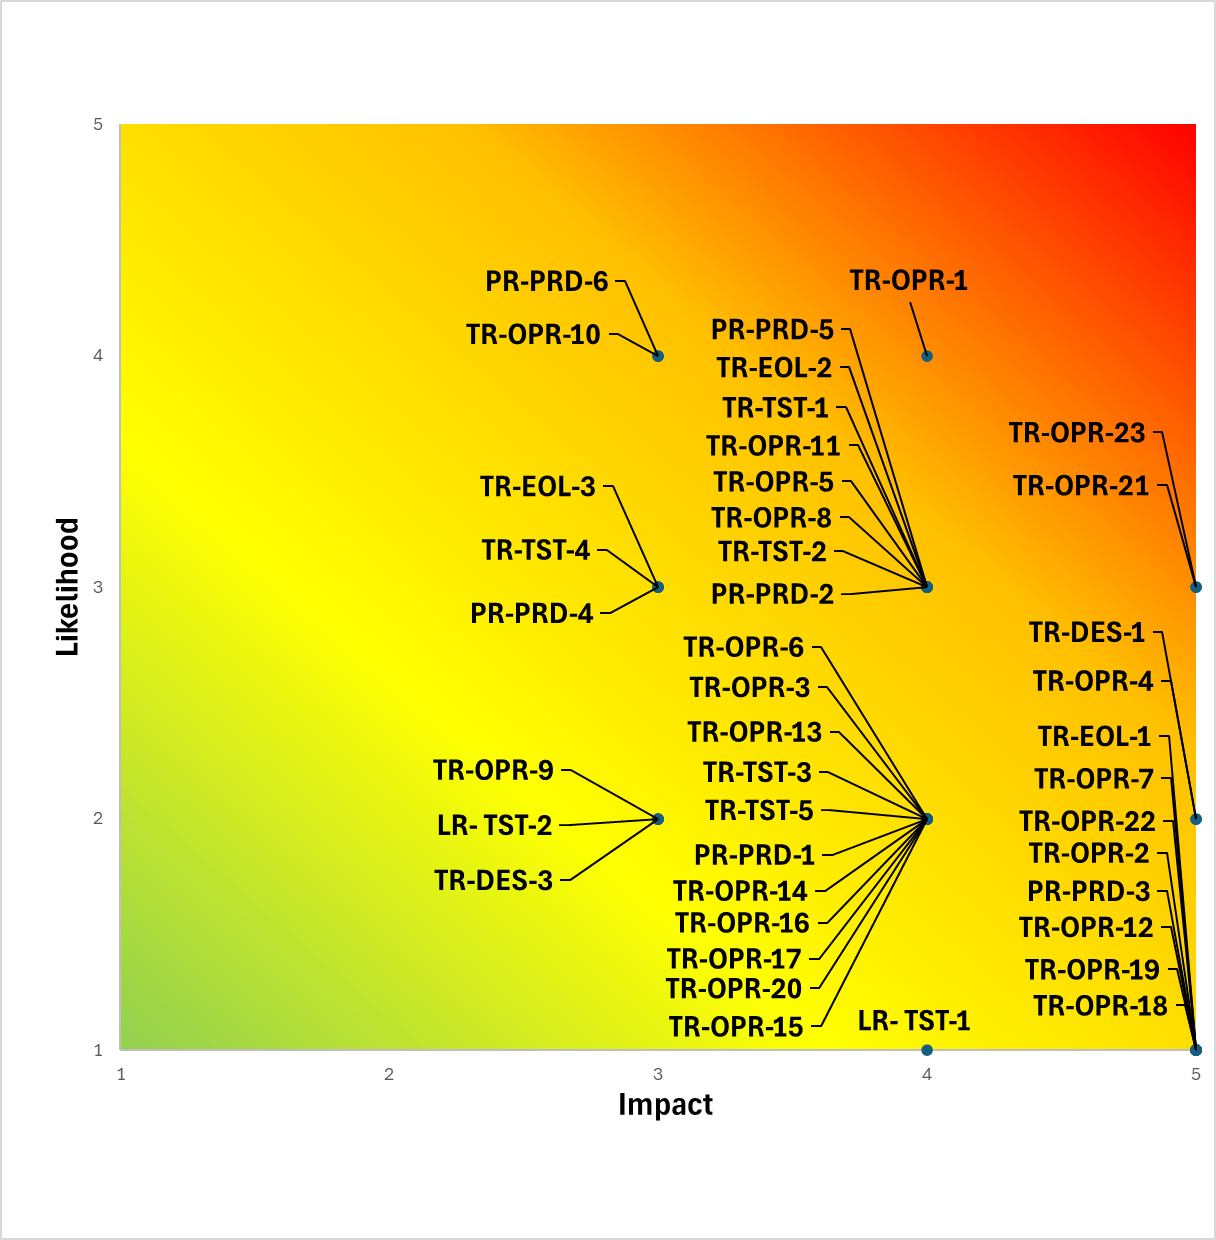
\includegraphics[width=\textwidth]{figures/AE3200 Risk map 1}
    \caption{Unmitigated risk map}
    \label{fig:risk_unm_tech}
  \end{subfigure}
  \hfill
  \begin{subfigure}[b]{0.49\textwidth} 
    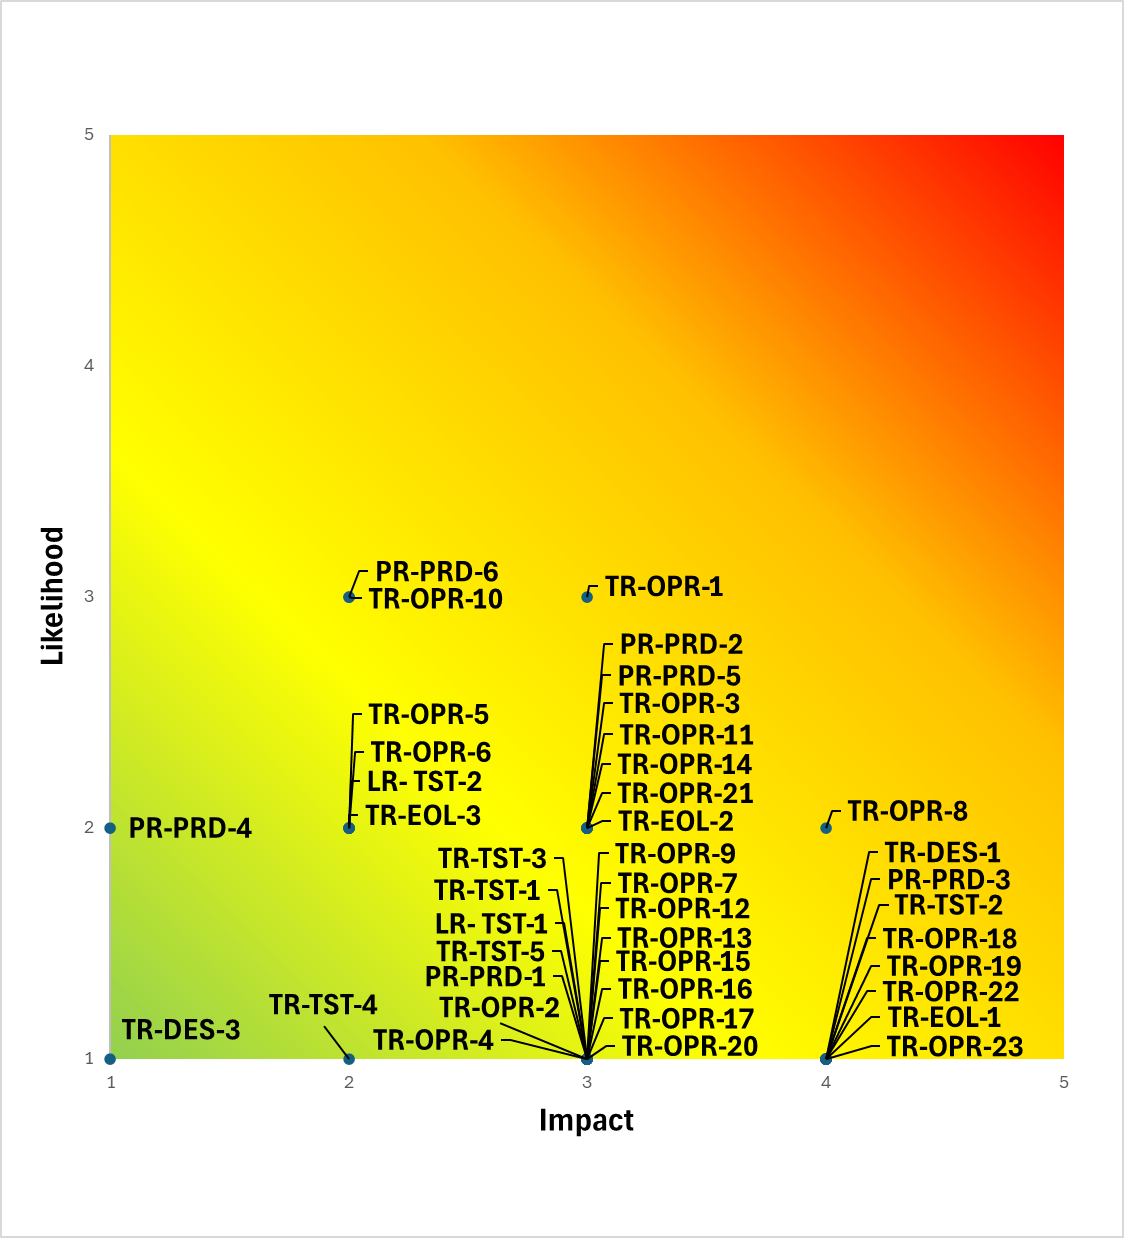
\includegraphics[width=\textwidth]{figures/AE3200 Risk map 2}
    \caption{Mitigated risk map}
    \label{fig:risk_mit_tech}
  \end{subfigure}
  \caption{Technical risk maps}
  \label{fig:Risk_map}
\end{figure}

\begin{table}[H]
\caption{Technical risks}
\label{tab:tech_risk_analysis}
\resizebox{\textwidth}{!}{%
\begin{tabular}{lcllccS[table-format=1.1,round-mode=places,round-precision=1,round-pad=true]}
\toprule
\multirow{2}{*}{\textbf{Risk ID}}   & \multirow{2}{*}{\textbf{Period}}      & \multirow{2}{*}{\textbf{Risk Description}}                                 & \multirow{2}{*}{\textbf{Impact Description}}                                            & \multicolumn{3}{c}{\textbf{Unmitigated Risk}}\\
          &             &                                                  &                                                               & \textbf{Likelihood}      & \textbf{Impact} & \textbf{Risk} \\ \midrule
TR-DES-1  & Design      & Deficient thrust generation                      & Unable to take-off                                            & 2                & 5      & \riskcolor{2}    \\
TR-DES-2  & Design      & Unavailable Additive Manufacturing facilities    & No 3D-model, so no visualisation of the design                & 2                & 3      & \riskcolor{1.2}  \\
PR-PRD-1  & Production  & Components too complex to manufacture            & Part cannot be manufactured, thus an unfeasible design        & 2                & 4      & \riskcolor{1.6}  \\
PR-PRD-2  & Production  & Subcontractor does not meet deadlines            & Delay of construction of the vehicle, testing and operations  & 3                & 4      & \riskcolor{2.4}  \\
PR-PRD-3  & Production  & Subcontractor's part not meeting requirements    & Failure of components results into a delay of production      & 1                & 5      & \riskcolor{1}    \\
PR-PRD-4  & Production  & Part manufacturing costs go over-budget          & Less budget for other segments or a budget shortfall         & 3                & 3      & \riskcolor{1.8}  \\
PR-PRD-5  & Production  & The required material is unavailable             & Delay of production                                           & 3                & 4      & \riskcolor{2.4}  \\
PR-PRD-6  & Production  & Increase in  material costs                      &    Less budget for other segments or a budget shortfall            & 4                & 3      & \riskcolor{2.4}  \\
LR- TST-1 & Testing     & \textit{Swing} is damaged during transportation           & Extra time and budget needed to repair the \textit{Swing}     & 1                & 4      & \riskcolor{0.8}  \\
LR- TST-2 & Testing     & Unavailable testing facility                     & Delay in testing or lack of physical test data                & 2                & 3      & \riskcolor{1.2}  \\
TR-TST-1  & Testing     & Hinge mechanism fails under wing loading         & Crash of prototype, and repair/redesign needed                & 3                & 4      & \riskcolor{2.4}  \\
TR-TST-2  & Testing     & Unrealistic simulation data                      & Under-performance or crash of the \textit{Swing}                            & 3                & 4      & \riskcolor{2.4}  \\
TR-TST-3  & Testing     & Vehicle violates the noise regulations           & Aero-acoustics have to be redesigned             & 2                & 4      & \riskcolor{1.6}  \\
TR-TST-4  & Testing     & No validation of the models                      & Uncertain if the design is valid and flyable                  & 3                & 3      & \riskcolor{1.8}  \\
TR-TST-5  & Testing     & Inaccurate stability analysis                    & Unstable during flight stages                         & 2                & 4      & \riskcolor{1.6}  \\
TR-OPR-1  & Operations  & Excessive maintenance& Unable to use vehicles, which increases delay and costs       & 4                & 4      & \riskcolor{3.2}  \\
TR-OPR-2  & Operations  & Power grid failure                               & Unable to charge the vehicles                                 & 1                & 5      & \riskcolor{1}    \\
TR-OPR-3  & Operations  & Damaged vertiport        & Unable to take off or land properly                           & 2                & 4      & \riskcolor{1.6}  \\
TR-OPR-4  & Operations  & Payload mass loaded is more than maximum          & Unable to take off or causing emergency                       & 2                & 5      & \riskcolor{2}    \\
TR-OPR-5  & Operations  & Sensors provide faulty or no data                & Faulty navigation or output by systems                        & 3                & 4      & \riskcolor{2.4}  \\
TR-OPR-6  & Operations  & Interference of  communications                  & Navigation interference                                       & 2                & 4      & \riskcolor{1.6}  \\
TR-OPR-7  & Operations  & Power system fails                               & Loss of thrust, navigation and control                        & 1                & 5      & \riskcolor{1}    \\
TR-OPR-8  & Operations  & Power drainage higher than expected in-flight    & Unable to fly full range and diversion to other vertiport & 3                & 4      & \riskcolor{2.4}  \\
TR-OPR-9  & Operations  & Navigation system fails                          & Unable to determine location and heading of the vehicle       & 2                & 3      & \riskcolor{1.2}  \\
TR-OPR-10 & Operations  & Damages infrastructure during take-off / landing & Increase in maintenance, repair costs and time                & 4                & 3      & \riskcolor{2.4}  \\
TR-OPR-11 & Operations  & Contact with animal                              & Possible fatal crash, involving casualties                    & 3                & 4      & \riskcolor{2.4}  \\
TR-OPR-12 & Operations  & Contact with human                               & Possible fatal crash, involving casualties                    & 1                & 5      & \riskcolor{1}    \\
TR-OPR-13 & Operations  & Folding mechanism malfunction during take-off    & Unable to transition to cruise                                & 2                & 4      & \riskcolor{1.6}  \\
TR-OPR-14 & Operations  & Folding mechanism malfunction during landing     & Unable to land vertically                                     & 2                & 4      & \riskcolor{1.6}  \\
TR-OPR-15 & Operations  & One engine failure in VTOL configuration                  & No yaw control, causing undesired spinning                    & 2                & 4      & \riskcolor{1.6}  \\
TR-OPR-16 & Operations  & Aileron failure                         & Limited roll control, oscillations may not be damped          & 2                & 4      & \riskcolor{1.6}  \\
TR-OPR-17 & Operations  & Ruddervator failure                     & Limited pitch and yaw control                                 & 2                & 4      & \riskcolor{1.6}  \\
TR-OPR-18 & Operations  & Battery pack failure                             & Total energy drop, not able to land vertically                & 1                & 5      & \riskcolor{1}    \\
TR-OPR-19 & Operations  & Autonomous system failure                          & Vehicle is not controlled                                     & 1                & 5      & \riskcolor{1}    \\
TR-OPR-20 & Operations  & Landing gear failure                             & Unable to land properly, causing an emergency landing         & 2                & 4      & \riskcolor{1.6}  \\
TR-OPR-21 & Operations  & Cybersecurity breach                             & Harmful intentions could result in a catastrophe              & 3                & 5      & \riskcolor{3}    \\
TR-OPR-22 & Operations  & In-flight fire                                   & Immediate emergency landing                         & 1                & 5      & \riskcolor{1}    \\
TR-OPR-23 & Operations  & Unforeseen flight conditions                     & Aircraft damaged and uncontrollable; emergency landing        & 3                & 5      & \riskcolor{3}    \\
TR-EOL-1  & End of life & Vehicle suffers total breakdown                  & Unable to be fulfil its required lifetime                     & 1                & 5      & \riskcolor{1}    \\
TR-EOL-2  & End of life & Unable to be recycled after its life             & Cannot meet  the set  sustainability goals                    & 3                & 4      & \riskcolor{2.4}  \\
TR-EOL-3  & End of life & Recycled components fail within 10 years         & Cannot meet  the set  sustainability goals                    & 3                & 3      & \riskcolor{1.8} \\ \bottomrule
\end{tabular}%
}
\end{table}

\section{Mitigation Strategies and Contingency Plans}
\label{sec:mitandcont}
To account for the established risks, mitigation strategies and contingency plans are in place to decrease the likelihood and impact, respectively.
These are all listed in \Cref{tab:risk_mit_conti}, and conclude the new risk factors in \Cref{tab:mit_risk_final}.
Also, a responsible team member related to the area of risk is appointed to monitor and manage the risk carefully.
With the newly acquired risk values, a mitigated risk map can be plotted in \Cref{fig:risk_mit_tech}.
The new risk map clearly illustrates a shift in risk likelihood and impact to better risk levels; hence, the mitigation strategies and contingency plans are successful.
In the map, it can be also seen that TR-OPR-1 and TR-OPR8 are still situated in the orange level, a moderate risk level, and thus should be monitored closely throughout the project.
The other risks have, however, decreased to a low to medium risk level (green and yellow),
which makes the project less susceptible to risks.


\begin{table}[H]
\centering
\caption{Mitigation strategies and contingency plans for risk management }
\label{tab:risk_mit_conti}
\resizebox{0.9\textwidth}{!}{%
\begin{tabular}{l|l|l}
\toprule
\textbf{Risk ID} & \textbf{Mitigation Strategy}                             & \textbf{Contingency Plan}                                   \\ \midrule
TR-DES-1         & Conduct thrust performance analysis                      & Alternative drop-in propulsion systems                      \\
TR-DES-3         & Reserve a place at the AM facility ahead of time         & Make use of personal 3D-printer                             \\
PR-PRD-1         & Elaborate use se of CAD and AM to visualise model        & Use different materials and  design options in CAD          \\
PR-PRD-2         & Constant monitoring and communication for deadlines      & Change contractors or impose costs                          \\
PR-PRD-3         & Use of test samples and prototypes before  production    & Change contractors or impose costs                          \\
PR-PRD-4         & Establish cost agreements in contracts                   & Include extra budget for unforeseen costs                   \\
PR-PRD-5         & Track material availability and buy in bulk              & Establish material replacements beforehand                  \\
PR-PRD-6         & Buy material in bulk, when the prices are within budget  & Include extra budget for unforeseen costs                   \\
LR- TST-1        & Elaborate inspection and testing before transportation   & Multiple spare parts available                              \\
LR- TST-2        & Clear communication with the testing facility            & Multiple possible testing facilities                        \\
TR-TST-1         & Use safety factors in loading analysis                   & Have spare hinge mechanism and wings available              \\
TR-TST-2         & Test subsystems thoroughly beforehand                    & Conduct limited testing and retrieve information            \\
TR-TST-3         & Extensive aeroacoustics analysis before testing          & Retrieve aeroacoustics data and redesign                    \\
TR-TST-4         & Use of validated models from similar research            & Perform subsystem testing  for validation                   \\
TR-TST-5         & Use of Computational Fluid Dynamics (CFD)                & Analyse and redesign control surfaces                       \\
TR-OPR-1         & Design low-maintenance parts                             & Look for extra or better trained maintenance staff          \\
TR-OPR-2         & Careful power grid structure design                      & Have diesel generators available as backup                  \\
TR-OPR-3         & Use of safety regulations near vertiports                & Have an emergency alternative vertiport available           \\
TR-OPR-4         & Conduct mass estimation before take-off                  & Decrease payload by unloading passengers/cargo              \\
TR-OPR-5         & Conduct frequent inspection and maintenance              & Emergency landing  procedure to nearest vertiport           \\
TR-OPR-6         & Implement redundant communication systems                & Emergency landing  procedure to nearest vertiport           \\
TR-OPR-7         & Conduct regular inspections of power systems             & Use backup power system or emergency landing                \\
TR-OPR-8         & Active  battery monitoring on power consumption          & Emergency landing  procedure to nearest vertiport           \\
TR-OPR-9         & Redundant navigation systems                             & Emergency landing  procedure to nearest vertiport           \\
TR-OPR-10        & Use of safety regulations and surroundings analysis      & Determine emergency procedures and protocols                \\
TR-OPR-11        & Use of animal detection system                           & Determine emergency procedures and protocols                \\
TR-OPR-12        & Strict flight safety protocols                           & Determine emergency procedures and protocols                \\
TR-OPR-13        & Conduct extensive testing and maintenance                & Emergency landing  procedure to nearest vertiport           \\
TR-OPR-14        & Conduct extensive testing and maintenance                & Emergency landing  procedure to nearest airport             \\
TR-OPR-15        & Test engines before each flight and regularly inspection & Programmed emergency landing  to nearest vertiport          \\
TR-OPR-16        & Conduct extensive testing and maintenance                & Use of thrust differential to induce roll and  land quickly \\
TR-OPR-17        & Conduct extensive testing and maintenance                & Use of thrust differential to induce yaw and land quickly   \\
TR-OPR-18        & Use  active cooling and a  battery management system     & Isolate faulty battery pack and land quickly  \\
TR-OPR-19        & Implement hard and software redundancy                   & Implement Fail-Safe Mode to transition the vehicle safely   \\
TR-OPR-20        & Perform regular system checks                            & Programmed emergency landing to nearest vertiport           \\
TR-OPR-21        & Encryption of data and communication                     & Pre-programmed emergency landing or manual override         \\
TR-OPR-22        & Use of fire-resistant materials and coatings             & Immediate descent and use of fire extinguishing system      \\
TR-OPR-23        & Use of weather forecasting and radar system              & Immediate descent or navigate out of  heavy weather         \\
TR-EOL-1         & Frequent maintenance and inspection                      & Investigate its cause                                       \\
TR-EOL-2         & Use of sustainable and recyclable materials              & Extensive analysis on recyclable materials                  \\
TR-EOL-3         & Frequent maintenance and inspection                      & Investigate its cause  \\
\bottomrule
\end{tabular}%
}
\end{table}


\begin{table}[H]
\centering
\caption{Mitigated risks}
\label{tab:mit_risk_final}
\resizebox{0.8\textwidth}{!}{%
\begin{tabular}{lcccc|lcccc}
\toprule
\multicolumn{1}{c}{\textbf{Risk ID}} & \textbf{Responsible} & \textbf{Likelihood} & \textbf{Impact} & \textbf{Risk} & \multicolumn{1}{c}{\textbf{Risk ID}} & \textbf{Responsible} & \textbf{Likelihood} & \textbf{Impact} & \textbf{Risk} \\ \midrule
TR-DES-1         & P\&P DC                     & 1                             & 4                                      & \riskcolor{0.8}  & TR-OPR-7         & P\&P DC                     & 1                             & 3                                      & \riskcolor{0.6}  \\
TR-DES-3         & CADM                        & 1                             & 1                                      & \riskcolor{0.2}  & TR-OPR-8         & C\&S DC                     & 2                             & 4                                      & \riskcolor{1.6}  \\
PR-PRD-1         & CADM                        & 1                             & 3                                      & \riskcolor{0.6}  & TR-OPR-9         & C\&S DC                     & 1                             & 3                                      & \riskcolor{0.6}  \\
PR-PRD-2         & CM                          & 2                             & 3                                      & \riskcolor{1.2}  & TR-OPR-10        & FP DC                       & 3                             & 2                                      & \riskcolor{1.2}  \\
PR-PRD-3         & CM                          & 1                             & 4                                      & \riskcolor{0.8}  & TR-OPR-11        & RM                          & 2                             & 3                                      & \riskcolor{1.2}  \\
PR-PRD-4         & CM                          & 2                             & 1                                      & \riskcolor{0.4}  & TR-OPR-12        & RM                          & 1                             & 3                                      & \riskcolor{0.6}  \\
PR-PRD-5         & RM                          & 2                             & 3                                      & \riskcolor{1.2}  & TR-OPR-13        & S\&M DC                     & 1                             & 3                                      & \riskcolor{0.6}  \\
PR-PRD-6         & CM                          & 3                             & 2                                      & \riskcolor{1.2}  & TR-OPR-14        & S\&M DC                     & 2                             & 3                                      & \riskcolor{1.2}  \\
LR- TST-1        & SE                          & 1                             & 3                                      & \riskcolor{0.6}  & TR-OPR-15        & P\&P DC                     & 1                             & 3                                      & \riskcolor{0.6}  \\
LR- TST-2        & CO                          & 2                             & 2                                      & \riskcolor{0.8}  & TR-OPR-16        & C\&S DC                     & 1                             & 3                                      & \riskcolor{0.6}  \\
TR-TST-1         & S\&M DC                     & 1                             & 3                                      & \riskcolor{0.6}  & TR-OPR-17        & C\&S DC                     & 1                             & 3                                      & \riskcolor{0.6}  \\
TR-TST-2         & QAO                         & 1                             & 4                                      & \riskcolor{0.8}  & TR-OPR-18        & P\&P DC                     & 1                             & 4                                      & \riskcolor{0.8}  \\
TR-TST-3         & Aero DC                     & 1                             & 3                                      & \riskcolor{0.6}  & TR-OPR-19        & C\&S DC                     & 1                             & 4                                      & \riskcolor{0.8}  \\
TR-TST-4         & SM                          & 1                             & 2                                      & \riskcolor{0.4}  & TR-OPR-20        & FP DC                       & 1                             & 3                                      & \riskcolor{0.6}  \\
TR-TST-5         & Aero DC                     & 1                             & 3                                      & \riskcolor{0.6}  & TR-OPR-21        & C\&S DC                     & 2                             & 3                                      & \riskcolor{1.2}  \\
TR-OPR-1         & CM                          & 3                             & 3                                      & \riskcolor{1.8}  & TR-OPR-22        & FP DC                       & 1                             & 4                                      & \riskcolor{0.8}  \\
TR-OPR-2         & P\&P DC                     & 1                             & 3                                      & \riskcolor{0.6}  & TR-OPR-23        & FP DC                       & 1                             & 4                                      & \riskcolor{0.8}  \\
TR-OPR-3         & QAO                         & 2                             & 3                                      & \riskcolor{1.2}  & TR-EOL-1         & PM                          & 1                             & 4                                      & \riskcolor{0.8}  \\
TR-OPR-4         & S\&M DC                     & 1                             & 3                                      & \riskcolor{0.6}  & TR-EOL-2         & SO                          & 2                             & 3                                      & \riskcolor{1.2}  \\
TR-OPR-5         & C\&S DC                     & 2                             & 2                                      & \riskcolor{0.8}  & TR-EOL-3         & SO                          & 2                             & 2                                      & \riskcolor{0.8}  \\
TR-OPR-6         & C\&S DC                     & 2                             & 2                                      & \riskcolor{0.8}  &                  &                             &                               &                                        &       \\
\bottomrule
\end{tabular}%
}
\end{table}
